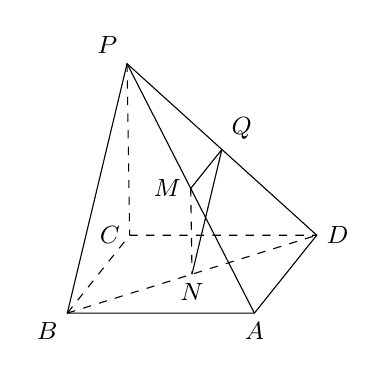
\begin{tikzpicture}[scale=.66, every node/.style={font=\small}]
  \coordinate (B) at (0,0);
  \coordinate (A) at (3.6,0);
  \coordinate (D) at (4.8,1.5);
  \coordinate (C) at (1.2,1.5);
  \coordinate (P) at (1.15,4.8);
  \coordinate (M) at (2.375,2.4);
  \coordinate (N) at (2.4,.75);
  \coordinate (Q) at (2.975,3.15);

  \draw[dashed] (B)--(C)--(D) (B)--(D) (P)--(C);
  \draw (B)--(A)--(D)--(P)--cycle;
  \draw (P)--(A) (M)--(Q) (N)--(Q);
  \draw[dashed] (M)--(N);

  \node[below left] at (B) {$B$};
  \node[below] at (A) {$A$};
  \node[right] at (D) {$D$};
  \node[left] at (C) {$C$};
  \node[above left] at (P) {$P$};
  \node[left] at (M) {$M$};
  \node[below] at (N) {$N$};
  \node[above right] at (Q) {$Q$};
\end{tikzpicture}
